\documentclass[12pt]{article}
 
\usepackage[margin=1in]{geometry} 
\usepackage{amsmath,amsthm,amssymb}
\usepackage{graphicx} 


\newcommand{\N}{\mathbb{N}}
\newcommand{\Z}{\mathbb{Z}}
 
\newenvironment{problem}[2][Problem]{\begin{trivlist}
\item[\hskip \labelsep {\bfseries #1}\hskip \labelsep {\bfseries #2.}]}{\end{trivlist}}
\newenvironment{lemma}[2][Lemma]{\begin{trivlist}
\item[\hskip \labelsep {\bfseries #1}\hskip \labelsep {\bfseries #2.}]}{\end{trivlist}}
\newenvironment{exercise}[2][Exercise]{\begin{trivlist}
\item[\hskip \labelsep {\bfseries #1}\hskip \labelsep {\bfseries #2.}]}{\end{trivlist}}

\newenvironment{question}[2][Question]{\begin{trivlist}
\item[\hskip \labelsep {\bfseries #1}\hskip \labelsep {\bfseries #2.}]}{\end{trivlist}}
\newenvironment{corollary}[2][Corollary]{\begin{trivlist}
\item[\hskip \labelsep {\bfseries #1}\hskip \labelsep {\bfseries #2.}]}{\end{trivlist}}

\usepackage{indentfirst}
\linespread{1.2}     % 调整间距
\setlength{\parindent}{0pt}

\begin{document}

 
% --------------------------------------------------------------
%                         Start here
% --------------------------------------------------------------
 
\title{Homework 1 DS-GA 1002 }%replace X with the appropriate number
\author{Yuhao Zhao\\ %replace with your name
N17578783} %if necessary, replace with your course title
 
\maketitle
 
\begin{problem}{1} 
%You can use theorem, exercise, problem, or question here.  Modify x.yz to be whatever number you are proving
\end{problem}
(a). If each of the friends decided to go independently, the number of people come can be modeled by a Binomial distribution, i.e Bin(5,0.1).\\
Therefore, the probability of three people come is ${5 \choose 3} \times 0.1^3 \times 0.9^2 \approx 0.0081$ 
\\

b) Let $S_i $ be the event that the friend i comes. The probability of no one comes is $1- P(U_iS_i)$, By the Union Bound theorem, $P(U_iS_i)  \leq \sum_{i }^{} P(S_i) = 0.1\times 5 = 0.5$, $1- P(U_iS_i) \geq 1-0.5 = 0.5$. Thus the lower bound is 0.5
 

\begin{problem}{2}
\end{problem}
(a) Let X be the event that Joe has the disease, and Y be the event that the test is positive. In particular, X follows a Bernoulli distribution.\\
P(Y) = P(someone has the disease, test positive)+P(no one has the disease, test positive )
		= (1- ${10 \choose 10} 0.8^{10}$)0.9 + 0.1${10 \choose 10}0.8^{10} \approx 0.8141$\\
Since P($X|Y$) $\times$ P(Y) = $P(Y|X) \times P(X)$\\
 P($X|Y$) = $\frac{P(Y|X) \times P(X)}{P(Y)}$ = $\frac{0.9 \times 0.2}{0.8141} \approx  0.2211$ \\
 
(b) Let A be the event that test is positive, B be the event that Joe has the disease, and C be the event that fridge is broken. We need to find out the relation of $P(A,B|C)$ with $P(A|C) \times P(B|C)$\\
$P(A,B|C) = \frac{P(A,B,C)}{P(C)} = \frac{P(C)P(B|C)P(A|B,C)}{P(C)}  = P(B|C)P(A|B,C)$\\
Thus, we just need to compare $P(A|C)$ and $P(A|B,C)$
%We assume that B and C are independent, this is reasonable because whether Joe has the disease should have no relation to whether the fridge is down.\\
%Therefore $P(B|A,C) = P(B|A) = 0.8844$\\
%$P(B|C)  = P(B) = 0.2$ By our assumption.\\
$P(A|C) = 1 , P(A|B,C) = 1$
Since $P(A|B,C) = P(A|C)$, the event A is independent of B given C.\\

(c) Define event A and C as part b.\\
$P(C|A) = \frac{P(A|C)P(C)}{P(A)} = \frac{1 \times 0.4}{0.6\times 0.8141 + 0.4 \times 1} \approx 0.4502$\\

\begin{problem}{3}
\end{problem}

%Since the car breaks down independently. The probability of breaking  down in the k'th drive is simply $\frac{1}{4}$\\
%Let breaking down in the k'+k drive be event A. $P(A|E) = \frac{P(A,E)}{P(E)}$. A and E are independent because the car breaks down independently. Whether the car breaks down in the first k drives has no influences on whether the car would break down in the k+k' drive.\\
%Therefore, $P(A|E) = P(A) = \frac{1}{4} $\\
%Therefore, the probability that the car breaks down in the k'th drive is equal to the probability of that it breaks down in th (k+k')th drive given E.\\
%This implies that the distribution of waiting time until the car breaks is memoryless,i.e $P (T \leq t) = P (T \leq t_0 + t| T > t_0), $
 (a) The probability of breaking  down for the first time in the k'th drive is $(\frac{3}{4})^{k'-1}\times \frac{1}{4} = \frac{3^{k'-1}}{4^{k'}}$\\
Let breaking down first time in the k'+k drive be event A. $P(A|E) = \frac{P(A,E)}{P(E)}$.\\
Since the break at $t_i$ is independent from the break at $t_j$,$E \subset A $, $P(A,E) = P(A) = (\frac{3}{4})^{k+k'-1}\times \frac{1}{4}$, $\frac{P(A,E)}{P(E)} = \frac{(\frac{3}{4})^{k+k'-1}\times \frac{1}{4}}{(\frac{3}{4})^{k} } = \frac{3^{k'-1}}{4^{k'}}$\\
Therefore, the probability that the car breaks down in the k'th drive is equal to the probability of that it breaks down in th (k+k')th drive given E.\\
This implies that the distribution of waiting time until the car breaks is memoryless,i.e $P (T \leq t) = P (T \leq t_0 + t| T > t_0), $\\


(b) P = ${k \choose n } \times (\frac{1}{4})^{n} \times (\frac{3}{4})^{k-n} $\\

(c) P =  ${k-1 \choose n-1} \times (\frac{1}{4})^{n-1} \times (\frac{3}{4})^{k-n} \times \frac{1}{4}$\\

(d) The probability of breaking  down first time in the k'th drive is :\\
$\prod_1^{k'-1} 2^{-n} \times (1 - 2^{-k'}) = (1 - 2^{-k'})\times 2^{-\frac{k'(k'-1)}{2}}   \quad eqn.1$\\
The probability of breaking down first time in the k+k' the drive given  E is:\\ $\frac{\prod_{1}^{k'+k-1}2^{-n}\times(1 - 2^{-k'-k})}{\prod_{1}^{k} 2^{-n}} =\frac{2^{\frac{-(k'+k)(k'+k-1)}{2}}\times(1 -2^{-k'-k})}{2^{\frac{-(1+k)k}{2}}}  \quad eqn.2$\\
We notice that in eqn.2 there is a cross term $k'k$, while in eqn.1 there is no k terms. eqn.2 and eqn.1 are not equal. This means that the distribution of waiting time until the car breaks under this model is not memoryless. This model is more realistic, since the car is more probable to break with longer driving time

\begin{problem}{4}
\end{problem}

(a)  Let T be the number of hours it takes to get a reading indicating the particle has decayed, and X be the actual time when the particle decayed.\\
$P(T = t) = P(X \in [t-1,t]) = \int_{t-1}^{t} \lambda e^{-\lambda x}dx  = -e^{-\lambda x}|_{t-1}^{t} = e^{-\lambda (t - 1)} - e^{-\lambda t} $\\

(b) The distribution of error $D,P(D \in [0, \delta])$ is just the sum of all probability that the decay happened $\delta$ hours ($\delta$ $<$ 1 ) prior to any integer time T  : \\
\begin{center}
	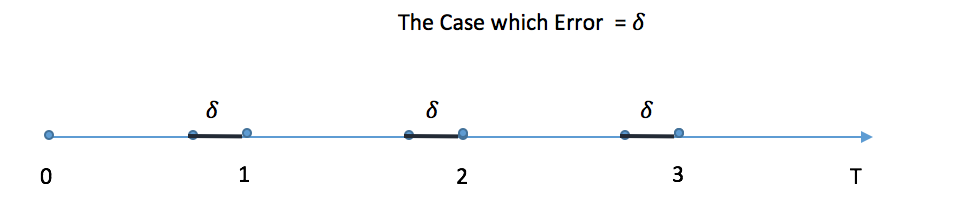
\includegraphics[height=1in]{p1} 
\end{center}
$P(D \in [0,\delta] ) = \sum_{n =1}^{\infty} \int_{n- \delta}^{n} \lambda e^{-\lambda x}dx =  \sum_{n =1}^{\infty} (- e^{-\lambda x}|_{n- \delta}^{n} ) = \sum_{n =1}^{\infty} (e^{-\lambda(n- \delta)} -e^{-n\lambda}) \\=  \sum_{n =1}^{\infty} (e^{-\lambda  n} (e^{\lambda  \delta}-1))  =   (e^{\lambda  \delta}-1) \sum_{n =1}^{\infty} (e^{-\lambda})^n$\\
Since for exponential distribution $\lambda >0 ,  e^{ - \lambda} <1$. Thus  $\sum_{n =1}^{\infty} (e^{-\lambda})^n$ is summable which is $\lim\limits_{n\to \infty}(e^{-\lambda})\frac{1 - e^{-n\lambda}}{1 - e^{-\lambda}} = \frac{e^{-\lambda}}{1- e^{-\lambda}}$\\
Therefore,$ P(D \in [0,\delta]) = \frac{e^{-\lambda}}{1- e^{-\lambda}}  (e^{\lambda  \delta}-1) $\\
%To solve C, we need to solve $\int_{0}^{1}  \frac{e^{-\lambda}}{1- e^{-\lambda}}  (e^{\lambda  \delta}-1) d\delta= C ,  \frac{e^{-\lambda}}{1- e^{-\lambda}} ( \frac{e^{\lambda\delta}}{\lambda} - \delta)|_0^1  = C$ \\
%$C =\frac{e^{-\lambda}}{1- e^{-\lambda}} (\frac{e^{\lambda }-1}{\lambda} -1)  = (\frac{1}{\lambda} - \frac{e^{-\lambda}}{1- e^{-\lambda}})$ \\
The pdf of E is the derivative of cdf which is :
$\frac{\lambda e^{-\lambda(1 - \delta)}}{1- e^{-\lambda}}  $\\

\begin{problem}{5}
\end{problem}
(a)  The CDF of W is $P(W<w) = P(F_Y(Y) < w )$\\
Since $F_Y$ is invertible, $P(F_Y(Y) < w ) = P(Y< F^{-1}_Y(w))$, this is , by definition of CDF, $F(F_Y^{-1}(w)) = w$.\\
Therefore we have $P(W<w)  = w$\\

(b) Let $T = F^{-1}_X(W)$, the CDF of T is $P(T<t) = P(F^{-1}_X(W)<t)  = P(W<F_X(t))$. Since we know the cdf of W is w. $P(W<F_X(t)) = F_X(t)$. The CDF of T and CDF of X are identical.\\

(c)  Since $F_Y$ is a CDF, it's non-decreasing, and right continuous. If $F_Y$ is not invertible, that means for a fixed constant w all the values of y such that $F_Y (y)$ = w belong to a closed interval
[a(w), b(w)], $F_Y$ is flat in this interval. We can still do the above even though $F_Y$ is not invertible. In particular, we can first omit the interval where $F_Y$ is not invertible and find the inverse. In the interval [a(w),b(w)], the inverse function is just a discontinuous jump from a(w) to b(w).  \\

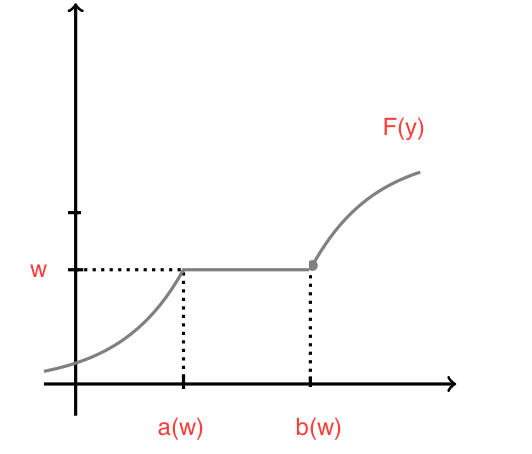
\includegraphics[height=2in]{p2}
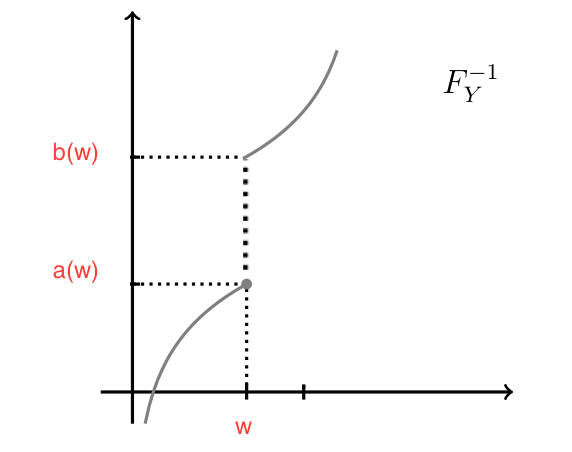
\includegraphics[height=2in]{p3}
 


 
\end{document}